\section{任务一}

本任务要求寻找除题目给定差分之外的高概率四轮差分。题目给出的差分为
\[
    (0x0,0x0,0x0,0x1)
    \xrightarrow{\text{4轮}}
    (0x0,0x0,0x0,0x1),
\]
也可以写成
\[
    0x0001\xrightarrow{\text{4轮}}0x0001.
\]

\subsection{直接穷举思路}

对于固定的输入差分 $\alpha$，可以遍历所有 $2^{16}$ 个 16 比特明文 $x$，构造有序明文对 $(x,x\oplus\alpha)$，然后分别进行四轮 CipherFour 加密。若最终密文差分为 $\beta$，则将对应计数加一。因此，固定输入、输出差分的概率为
\[
    P(\alpha\rightarrow\beta)
    =
    \frac{\#\{x:E(x)\oplus E(x\oplus\alpha)=\beta\}}{2^{16}}.
\]

对于每一个非零输入差分，共有 $2^{16}$ 个有序明文对；如果不区分明文对的顺序，则有 $2^{15}$ 个无序明文对。若对全部 $2^{16}-1$ 个非零输入差分都进行穷举，需要处理约 $2^{32}$ 组明文对，计算开销较大。因此，程序使用 S 盒差分分布表（DDT）对差分进行动态规划。

\subsection{S盒差分分布表}

CipherFour 使用一个 4 进 4 出的 S 盒。对于输入差分 $\alpha$ 和输出差分 $\beta$，DDT 定义为
\[
    \mathrm{DDT}[\alpha][\beta]
    =
    \#\left\{x\in\{0,1,\ldots,15\}:
    S(x)\oplus S(x\oplus\alpha)=\beta\right\}.
\]

因此，单个 S 盒的差分传播概率为
\[
    T[\alpha][\beta]
    =
    \frac{\mathrm{DDT}[\alpha][\beta]}{16}
    =
    \frac{\mathrm{DDT}[\alpha][\beta]}{2^4}.
\]

代码中的 DDT 计算如下：
\begin{lstlisting}
for diff_in in range(16):
    for value in range(16):
        diff_out = S[value] ^ S[value ^ diff_in]
        diff_table[diff_in][diff_out] += 1
\end{lstlisting}

其中，\texttt{diff\_table[diff\_in][diff\_out]} 保存输入差分为 \texttt{diff\_in}、输出差分为 \texttt{diff\_out} 的出现次数。

\subsection{一轮差分传播}

一个 16 比特差分可以拆成四个半字节：
\[
    \Delta=(a_0,a_1,a_2,a_3).
\]

若四个 S 盒的输出差分为
\[
    \Gamma=(b_0,b_1,b_2,b_3),
\]
则在固定当前差分的条件下，四个 S 盒同时发生该传播的概率为
\[
    Q(\Delta,\Gamma)
    =
    \prod_{i=0}^{3}T[a_i][b_i].
\]

例如，输入差分 $0x0001=(0,0,0,1)$ 时，前三个 S 盒的输入差分为 0，并且
\[
    T[0][0]=1.
\]
只有最后一个 S 盒产生分支。对于本实验使用的 S 盒，输入差分 1 可以传播为输出差分 1、2、5，其概率分别为 $1/2$、$1/4$、$1/4$。因此，经过 S 盒层后可能得到
\[
    0x0001\ (1/2),\qquad
    0x0002\ (1/4),\qquad
    0x0005\ (1/4).
\]

代码中的 \texttt{score} 保存四个半字节的联合概率分布，其形状为
\[
    (\text{batch},16,16,16,16).
\]
处理某一个半字节时，程序计算
\[
    F_{\mathrm{new}}(\beta)
    =
    \sum_{\alpha=0}^{15}
    F_{\mathrm{old}}(\alpha)T[\alpha][\beta].
\]

这对应代码中的矩阵乘法：
\begin{lstlisting}
score_matrix = moved_score.reshape(-1, 16)
updated_score = score_matrix @ probability_table
\end{lstlisting}

程序依次处理四个 S 盒：
\begin{lstlisting}
for position in range(4):
    score = update_one_sbox_distribution(
        score, probability_table, position
    )
\end{lstlisting}

对于一个确定的当前 16 比特差分，这一过程等价于四个 S 盒概率的乘积；当当前状态本身是多个差分状态的概率混合时，程序还会对所有前驱状态的概率进行求和，因此需要保存四个半字节的联合分布，而不能只分别保存四个边缘概率。

四个 S 盒处理完成后，将得到的 16 比特差分经过 P 置换。代码预先计算所有 16 比特状态的置换结果：
\begin{lstlisting}
permutation = np.array(
    [P_box(value) for value in range(STATE_SIZE)],
    dtype=np.int32,
)
\end{lstlisting}

由于 P 是比特置换，满足
\[
    P(X)\oplus P(Y)=P(X\oplus Y),
\]
因此可以直接对差分状态进行 P 置换。经过 P 置换后的差分分布作为下一轮的输入。

\subsection{四轮动态规划}

设初始输入差分为 $\alpha$，经过 $r$ 轮后的差分分布为 $D_r^{(\alpha)}$。初始时只有输入差分本身的概率为 1：
\[
    D_0^{(\alpha)}(\Delta)=
    \begin{cases}
        1,&\Delta=\alpha,\\
        0,&\Delta\ne\alpha.
    \end{cases}
\]

代码通过以下语句完成初始化：
\begin{lstlisting}
score[rows, nibble0, nibble1, nibble2, nibble3] = 1.0
\end{lstlisting}

记一轮四个 S 盒和 P 置换的差分转移概率为 $R(\Delta,\Delta')$，则每轮动态规划满足
\[
    D_{r+1}^{(\alpha)}(\Delta')
    =
    \sum_{\Delta}
    D_r^{(\alpha)}(\Delta)R(\Delta,\Delta').
\]

因此，四轮后的输出差分概率为
\[
    D_4^{(\alpha)}(\beta)
    =
    \sum_{\Delta_1,\Delta_2,\Delta_3}
    R(\alpha,\Delta_1)
    R(\Delta_1,\Delta_2)
    R(\Delta_2,\Delta_3)
    R(\Delta_3,\beta).
\]

这个求和包含了从输入差分 $\alpha$ 到输出差分 $\beta$ 的所有差分路线。代码的外层循环对应四轮传播：
\begin{lstlisting}
for _ in range(NUMBER_OF_ROUNDS):
    for position in range(4):
        score = update_one_sbox_distribution(
            score, probability_table, position
        )

    after_sbox = score.reshape(batch_size, STATE_SIZE)
    after_pbox[:, permutation] = after_sbox
    score = after_pbox.reshape(
        batch_size, 16, 16, 16, 16
    )
\end{lstlisting}

这里每一轮的输入和输出都是 16 比特差分状态的概率分布，不是具体的明文或密文。四轮循环结束后，\texttt{score} 中保存每个输入差分经过四轮后得到所有输出差分的概率。

\subsection{高概率差分的搜索}

程序从 \texttt{0x0001} 到 \texttt{0xFFFF} 遍历全部 $2^{16}-1$ 个非零输入差分，并将输入差分按 32 个一批进行处理，以降低内存开销。分批处理不会减少搜索范围。

对于每个输入差分 $\alpha$，四轮动态规划得到所有输出差分 $\beta$ 的概率分布。程序使用
\begin{lstlisting}
output_differences = np.argmax(
    output_distribution, axis=1
)
\end{lstlisting}
找到该输入差分对应的最大概率输出差分。随后，再在所有输入差分对应的候选结果中选择全局最大值。

题目要求排除 $0x0001\rightarrow0x0001$，因此代码只对输入差分 \texttt{0x0001} 的输出分布执行：
\begin{lstlisting}
candidate_distribution[
    EXCLUDED_OUTPUT_DIFFERENCE
] = 0.0
\end{lstlisting}
然后重新选择该输入差分对应的最佳输出差分。

\begin{figure}[H]
    \centering
    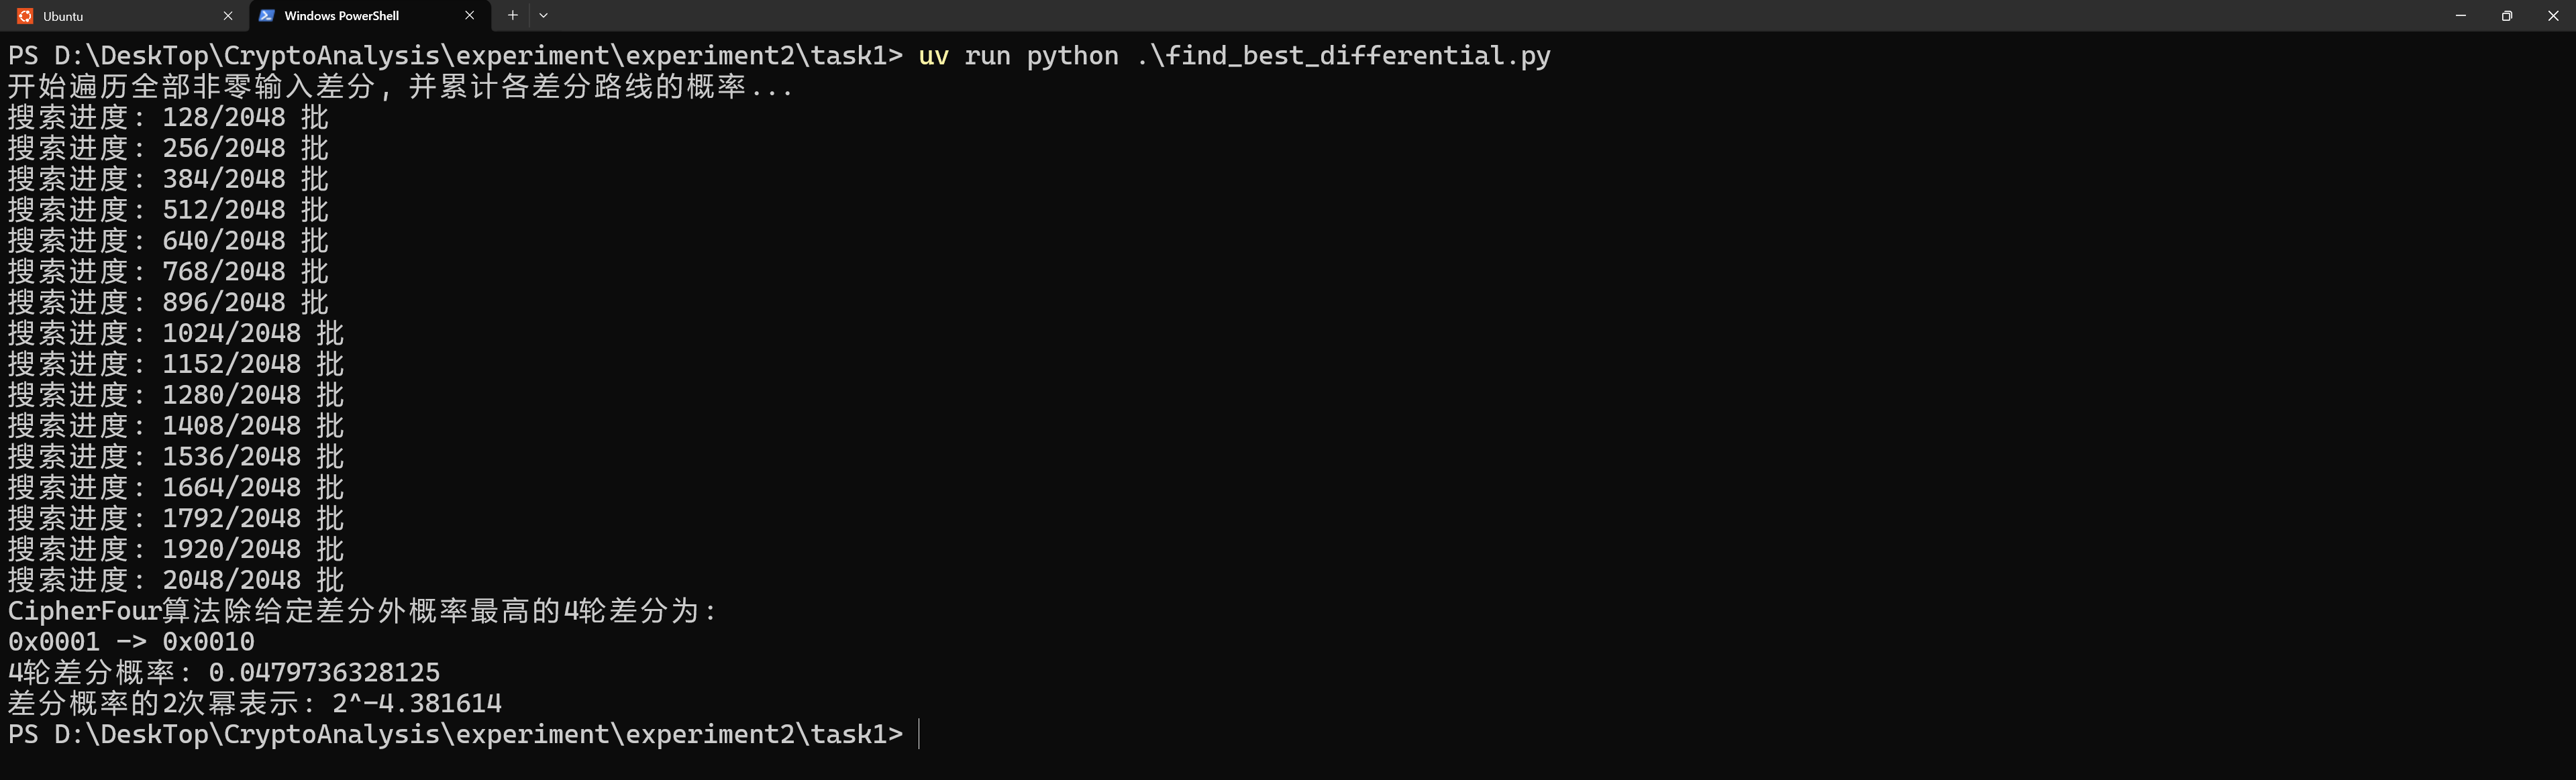
\includegraphics[width = 1\textwidth]{figures/task1_diffeientrial.png}
    \caption{寻找高概率差分}
\end{figure}

程序最终找到的四轮高概率差分为
\[
    (0x0,0x0,0x0,0x1)
    \longrightarrow
    (0x0,0x0,0x1,0x0),
\]
即
\[
    0x0001\longrightarrow0x0010.
\]

其基于 DDT 动态规划得到的四轮差分概率为
\[
    P(0x0001\rightarrow0x0010)
    =0.0479736328125
    \approx 2^{-4.381614}.
\]

这里计算的是连接相同输入、输出差分的所有差分路线的概率总和，而不是某一条单独差分路线的概率。后续任务二再通过枚举具体明文对，统计该输入、输出差分在固定 CipherFour 置换网络中的实际路线和频率。